\subsubsection{generation.roomgeneration}
    \textit{Roomgeneration} ist dafür verantwortlich einen Raum zu generieren, der eine Straße besitzt und so 
    in eine Rennstrecke eingebaut werdenkann. Diser kann komplett prozedural generiert werden, aus einem Asset bestehen.
    Um das zu bewerkstelligen wird eine Liste von Generatoren (\textit{AbstractRoomGenerator}) verwaltet, welche
    auf unterschiedliche Weise Räume erstellen.\par

    \begin{figure}[htbp]
        \centering
        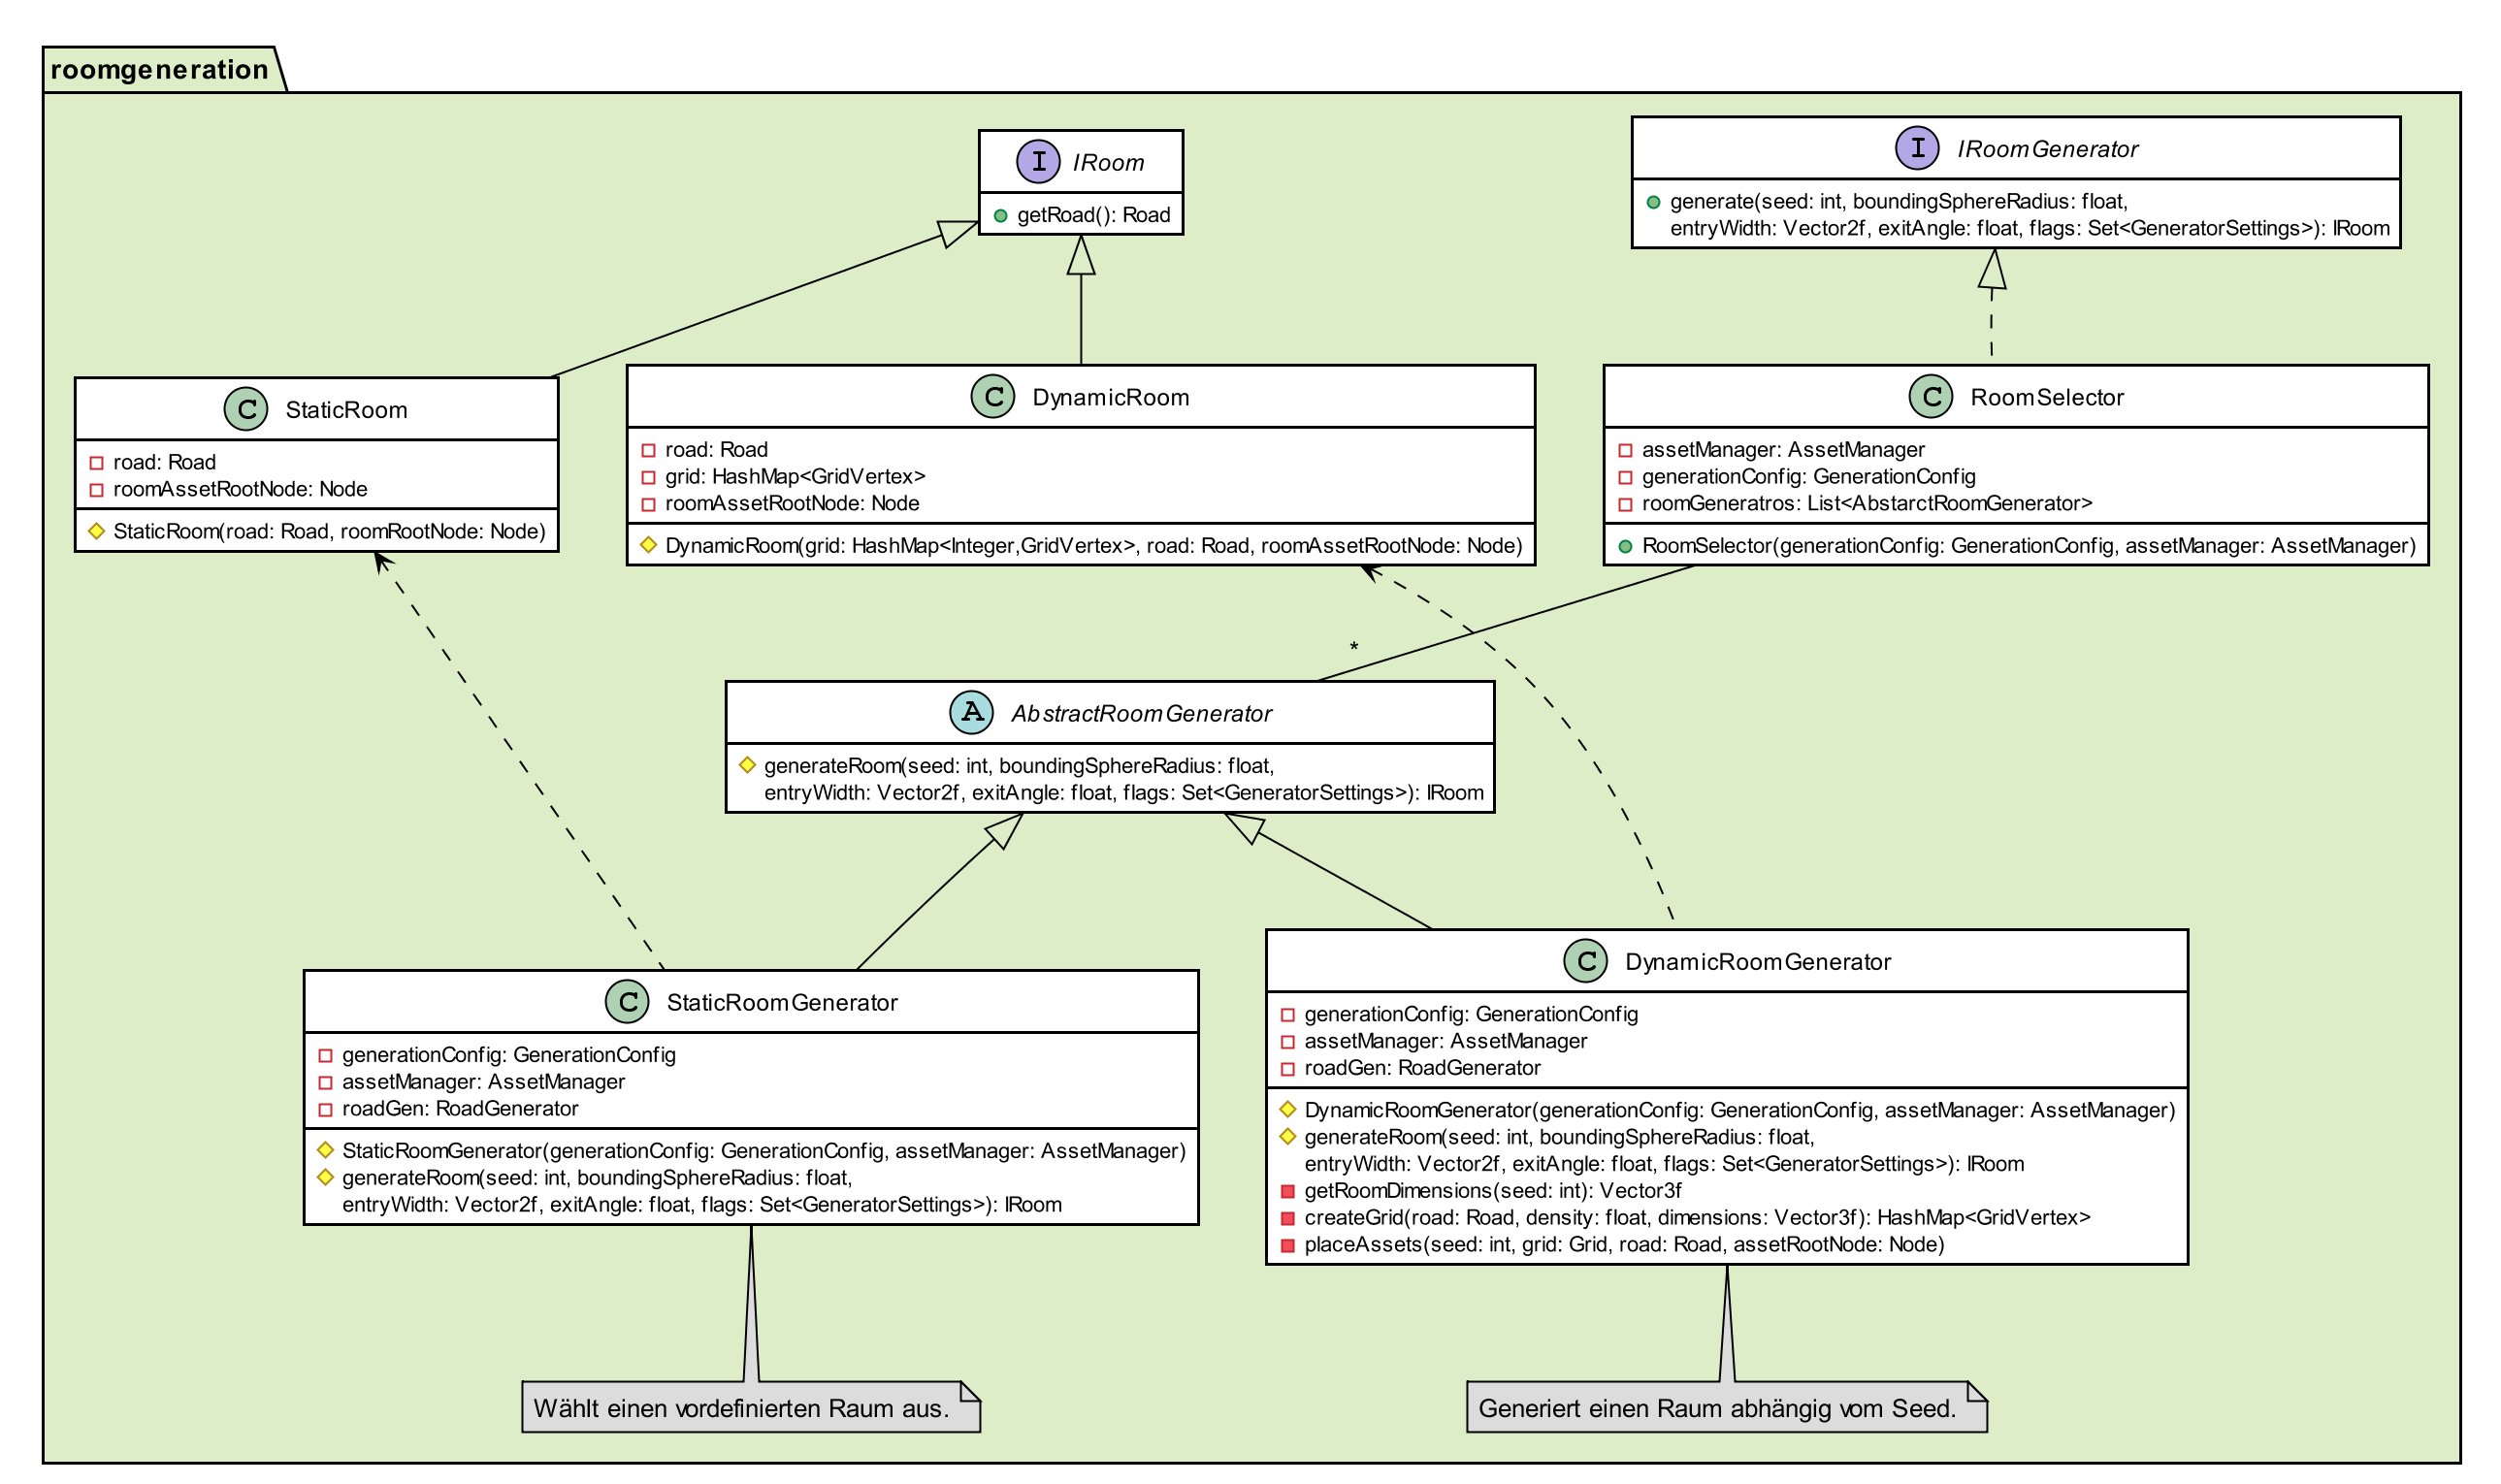
\includegraphics[width=\linewidth]{./Generierung/Bilder/roomgeneration.png}
        \caption{Klassendiagramm roomgeneration}
    \end{figure}

        \pagebreak
        \paragraph{\underline{IRoomGenerator}} \mbox{}\par
            Schnittstelle nach außen, um die Raumgenerieung anzustoßen, hierbei kann kein Einfluss auf die Art der Generierung 
            genommen werden.\par
            
            \textbf{Methoden}					
            \begin{itemize}
                \item  \textit{+ generate(int seed, float boundingSphereRadius,Vector2f entryWidth, float exitAngle, Set<GeneratorSettings> flags): IRoom}
                    \begin{leftbar}[0.9\linewidth]
                        Stößt den Generierungsprozess eines Raumes (\textit{IRoom}) an.\\
                        \textbf{@param seed} Zum bestimmen von Pseudozufallswerten.\\
                        \textbf{@param boundingSphereRadius} Definiert einen Kreis, indem der Raum bleiben muss, um seine Maße einzugrenzen.\\
                        \textbf{@param entryWidth} Bschreibt die Dimension des Eingangs.\\
                        \textbf{@param exitAngle} Bschreibt den Winkel zwischen Ein-/ und Ausgang.\\
                        \textbf{@param flags} Menge an Präferenzen, die zur Generierung übergegben werden.\\
                        \textbf{@return} Datenstruktur, die einen Raum repräsentiert.
                    \end{leftbar}   
            \end{itemize}
            
        
        
        \paragraph{\underline{RoomSelector}} \mbox{}\par
            Implementiert \textit{IRoomGenerator} führt jedoch keine echte Generierungan durch sondern hält ein Set von Generatoren (\textit{AbstractRoomGenerator}),
            von denen er jeweils einen auswählt, um durch diesen die Generierung ausführen zu lassen.\par
            
            \textbf{Attribute}
            \begin{itemize}
                \item  \textit{- AssetManager assetManager} 
                    \begin{leftbar}[0.9\linewidth]
                        Von \textit{JMonkey} vordefinierte Klasse, zum verwalten von Assets.
                    \end{leftbar}
                
                \item  \textit{- GenerationConfig generationConfig} 
                    \begin{leftbar}[0.9\linewidth]
                        Datenstruktur, die Parameter für die Generierung hält.
                    \end{leftbar}
                
                    \item  \textit{- List<AbstarctRoomGenerator> roomGeneratros} 
                    \begin{leftbar}[0.9\linewidth]
                        Datenstruktur, die Parameter für die Generierung hält.
                    \end{leftbar}
            \end{itemize}

            \textbf{Methoden}					
            \begin{itemize}
                \item  \textit{+ RoomSelector(GenerationConfig generationConfig, AssetManager assetManager)}
                    \begin{leftbar}[0.9\linewidth]
                        Konsrtuktor für \textit{RoomSelector}. Erstellt eine Menge an Generatoren des Typs \textit{AbstarctRoomGenerator} 
                        aus denen für die eigentliche Generierung jedes mal einer ausgewählt werden kann.\\
                        \textbf{@param generationConfig} Datenstruktur, die Parameter für die Generierung hält.\\
                        \textbf{@param assetManager} Von \textit{JMonkey} vordefinierte Klasse, zum verwalten von Assets.
                    \end{leftbar}   
            \end{itemize}
            
        
        
        \paragraph{\underline{AbstractRoomGenerator}} \mbox{}\par
            Definiert und implementiert die Grundfunktionalität, die jeder Generator eines \textit{IRoom} erfüllen muss.\par
            
            \textbf{Methoden}					
            \begin{itemize}
                \item  \textit{\# generateRoom(int seed, float boundingSphereRadius,Vector2f entryWidth, float exitAngle, Set<GeneratorSettings> flags): IRoom}
                    \begin{leftbar}[0.9\linewidth]
                        Stößt den Generierungsprozess eines Raumes (\textit{IRoom}) an.\\
                        \textbf{@param seed} Zum bestimmen von Pseudozufallswerten.\\
                        \textbf{@param boundingSphereRadius} Definiert einen Kreis, indem der Raum bleiben muss, um seine Maße einzugrenzen.\\
                        \textbf{@param entryWidth} Bschreibt die Dimension des Eingangs.\\
                        \textbf{@param exitAngle} Bschreibt den Winkel zwischen Ein-/ und Ausgang.\\
                        \textbf{@param flags} Menge an Präferenzen, die zur Generierung übergegben werden.\\
                        \textbf{@return} Datenstruktur, die einen Raum repräsentiert.
                    \end{leftbar}   
            \end{itemize}
        
        
        
        \paragraph{\underline{DynamicRoomGenerator}} \mbox{}\par
            Erweitert \textit{AbstractRoomGenerator} in durch eine konkrete Impementirung der \textit{generate()} Funktion.
            Hierbei wird ein Raum prozedural generiert, indem er aus verschiedenen Assets zusammen gesetzt wird.\par
            
            \textbf{Attribute}
            \begin{itemize}
                \item  \textit{- GenerationConfig generationConfig} 
                    \begin{leftbar}[0.9\linewidth]
                        Datenstruktur, die Parameter für die Generierung hält.
                    \end{leftbar}
                
                \item  \textit{- AssetManager assetManager} 
                    \begin{leftbar}[0.9\linewidth]
                        Von \textit{JMonkey} vordefinierte Klasse, zum verwalten von Assets.
                    \end{leftbar}
                
                \item  \textit{- IRoadGenerator roadGen} 
                    \begin{leftbar}[0.9\linewidth]
                        Ist für die Generierung eines Streckenverlaufs verantwortlich.
                    \end{leftbar}
            \end{itemize}

            \textbf{Methoden}					
            \begin{itemize}
                \item  \textit{\# DynamicRoomGenerator(GenerationConfig generationConfig, AssetManager assetManager)}
                    \begin{leftbar}[0.9\linewidth]
                        Konsrtuktor für \textit{DynamicRoomGenerator}.\\
                        \textbf{@param generationConfig} Datenstruktur, die Parameter für die Generierung hält.\\
                        \textbf{@param assetManager}  Von \textit{JMonkey} vordefinierte Klasse, zum verwalten von Assets.
                    \end{leftbar} 
            \end{itemize}
        
        
        \pagebreak
        \paragraph{\underline{StaticRoomGenerator}} \mbox{}\par
            Erweitert \textit{AbstractRoomGenerator} in durch eine konkrete Impementirung der \textit{generate()} Funktion.
            Hierbei wird jedoch lediglich ein Asset, das einen ganzen Raum repräsentiert, geladen.\par
                
            \textbf{Attribute}
            \begin{itemize}
                \item  \textit{- GenerationConfig generationConfig} 
                    \begin{leftbar}[0.9\linewidth]
                        Datenstruktur, die Parameter für die Generierung hält.
                    \end{leftbar}
                
                \item  \textit{- AssetManager assetManager} 
                    \begin{leftbar}[0.9\linewidth]
                        Von \textit{JMonkey} vordefinierte Klasse, zum verwalten von Assets.
                    \end{leftbar}
                
                \item  \textit{- IRoadGenerator roadGen} 
                    \begin{leftbar}[0.9\linewidth]
                        Ist für die Generierung eines Streckenverlaufs verantwortlich.
                    \end{leftbar}
            \end{itemize}

            \textbf{Methoden}					
            \begin{itemize}
                \item  \textit{\# StaticRoomGenerator(GenerationConfig generationConfig, AssetManager assetManager)}
                    \begin{leftbar}[0.9\linewidth]
                        Konsrtuktor für \textit{StaticRoomGenerator}.\\
                        \textbf{@param generationConfig} Datenstruktur, die Parameter für die Generierung hält.\\
                        \textbf{@param assetManager}  Von \textit{JMonkey} vordefinierte Klasse, zum verwalten von Assets.
                    \end{leftbar}  
            \end{itemize}
        
        
        
        \paragraph{\underline{IRoom}} \mbox{}\par
            Definiert die Grundfunktionalität der Datenstruktur eines Raums.\par

            \textbf{Methoden}					
            \begin{itemize}
                \item  \textit{+ generateSceneGraph(): Node}
                    \begin{leftbar}[0.9\linewidth]
                        Berechnet Scenegraph des Raums und gibt ihn zurück.\\
                        \textbf{@return}  Verwendet wie in \textit{JMonkey}, wird übergeben um den Tunnel in einer Szene darzustellen.
                    \end{leftbar}

                \item  \textit{+ getRoad(): Road}
                    \begin{leftbar}[0.9\linewidth]
                        Gibt die Straße (\textit{Road}), die durch den Raum verläuft, zurück.\\
                        \textbf{@return} Repräsentiert die Straße in dem Raum.
                    \end{leftbar}    
            \end{itemize}
        
        
        \pagebreak
        \paragraph{\underline{DynamicRoom}} \mbox{}\par
            Impementiert \textit{IRoom} und bildet somit eine konkrete Datenstruktur, die einen Raum, der prozedural generiert wurde, beschreibt.\par
            
            \textbf{Attribute}
            \begin{itemize}
                \item  \textit{- Road road} 
                    \begin{leftbar}[0.9\linewidth]
                        Datenstruktur die eine Straße, die durch den Raum verläuft, repräsentiert.
                    \end{leftbar}
                
                \item  \textit{- HashMap<GridVertex> grid} 
                    \begin{leftbar}[0.9\linewidth]
                        Das Gitter des Raumes, das verschiedene Stati pro \textit{GridVertex} speichert.
                    \end{leftbar}
                
                \item  \textit{- Node roomAssetRootNode} 
                    \begin{leftbar}[0.9\linewidth]
                        Verwendet wie in \textit{JMonkey}, hier sollen alle Objekte aus dem Raum angehängt werden.
                    \end{leftbar}
            \end{itemize}

            \textbf{Methoden}					
            \begin{itemize}
                \item  \textit{\# DynamicRoom(HashMap<Integer,GridVertex> grid, Road road, Node roomAssetRootNode)}
                    \begin{leftbar}[0.9\linewidth]
                        Konsrtuktor für \textit{DynamicRoom}.\\
                        \textbf{@param gird} Das Gitter des Raumes, das verschiedene Stati pro \textit{GridVertex} speichert.\\
                        \textbf{@param road} Repräsentiert die Straße, die durch den Raum verläuft.\\
                        \textbf{@param roomAssetRootNode} Verwendet wie in \textit{JMonkey}, hier sollen alle Objekte aus dem Raum angehängt werden.
                    \end{leftbar}   
            \end{itemize}
        
        
        \pagebreak
        \paragraph{\underline{StaticRoom}} \mbox{}\par
         Impementiert \textit{IRoom} und bildet somit eine konkrete Datenstruktur, die einen Raum, der aus einem Asset besteht, beschreibt.\par
            
            \textbf{Attribute}
            \begin{itemize}
                \item  \textit{- Road road} 
                    \begin{leftbar}[0.9\linewidth]
                        Datenstruktur, die die Straße, die durch den Raum verläuft repräsentiert.
                    \end{leftbar}
                
                \item  \textit{- Node roomRootNode} 
                    \begin{leftbar}[0.9\linewidth]
                        Verwendet wie in \textit{JMonkey}, hier sollen der Raum angehängt werden.
                    \end{leftbar}
            \end{itemize}

            \textbf{Methoden}					
            \begin{itemize}
                \item  \textit{\# StaticRoom(Road road, Node roomRootNode)}
                    \begin{leftbar}[0.9\linewidth]
                        Konsrtuktor für \textit{StaticRoom}.\\
                        \textbf{@param road} Repräsentiert die STraße, die durch den Raum verläuft.\\
                        \textbf{@param roomRootNode}  Verwendet wie in \textit{JMonkey}, hier sollen der Raum angehängt werden.
                    \end{leftbar}
 
            \end{itemize}

       
       
       
        
        
        
        